% Modelo de slides para projetos de disciplinas do Abel
\documentclass[aspectratio=169]{beamer}
\hypersetup{pdfpagemode=FullScreen}
\usetheme[progressbar=frametitle]{metropolis}
\usepackage{appendixnumberbeamer}
\usepackage[numbers,sort&compress]{natbib}
\usepackage{listings}
\bibliographystyle{plainnat}
\usepackage{listings}
\usepackage{hyperref}
\usepackage{booktabs}
\usepackage{tikz}
\usepackage{tikzpeople}
\usetikzlibrary{shapes,arrows}
\usepackage[scale=1]{ccicons}
% \usepackage{enumitem} % not compatible with enumerate in beamer class
\usepackage{xspace}
\newcommand{\themename}{\textbf{\textsc{metropolis}}\xspace}

\title{Reddit Cryptocurrency Comments Analysis}
% \subtitle{Subtítulo}
% \date{\today}
\date{March 31, 2022}
\author{Albin Aliu, François-Xavier Wicht \& Grégoire Rebstein}
\institute{Social Media Analytics}
% \titlegraphic{\hfill\includegraphics[height=1.5cm]{logo.pdf}}

\begin{document}

\maketitle

\begin{frame}{Agenda}
    \setbeamertemplate{section in toc}[sections numbered]
    \tableofcontents
\end{frame}
\section{Overview}
\begin{frame}[t]
    \frametitle{Overview}
    \begin{columns}
        \column{0.4\textwidth}
        \begin{itemize}
            \item The main idea is to find a link between the activity in cryptocurrency subreddits and the price of \textbf{Bitcoin}.
            \item For that we modeled the data in an appropriate way and ran several algorithms seen in class.
        \end{itemize}
%        \vspace{1.0cm}
%        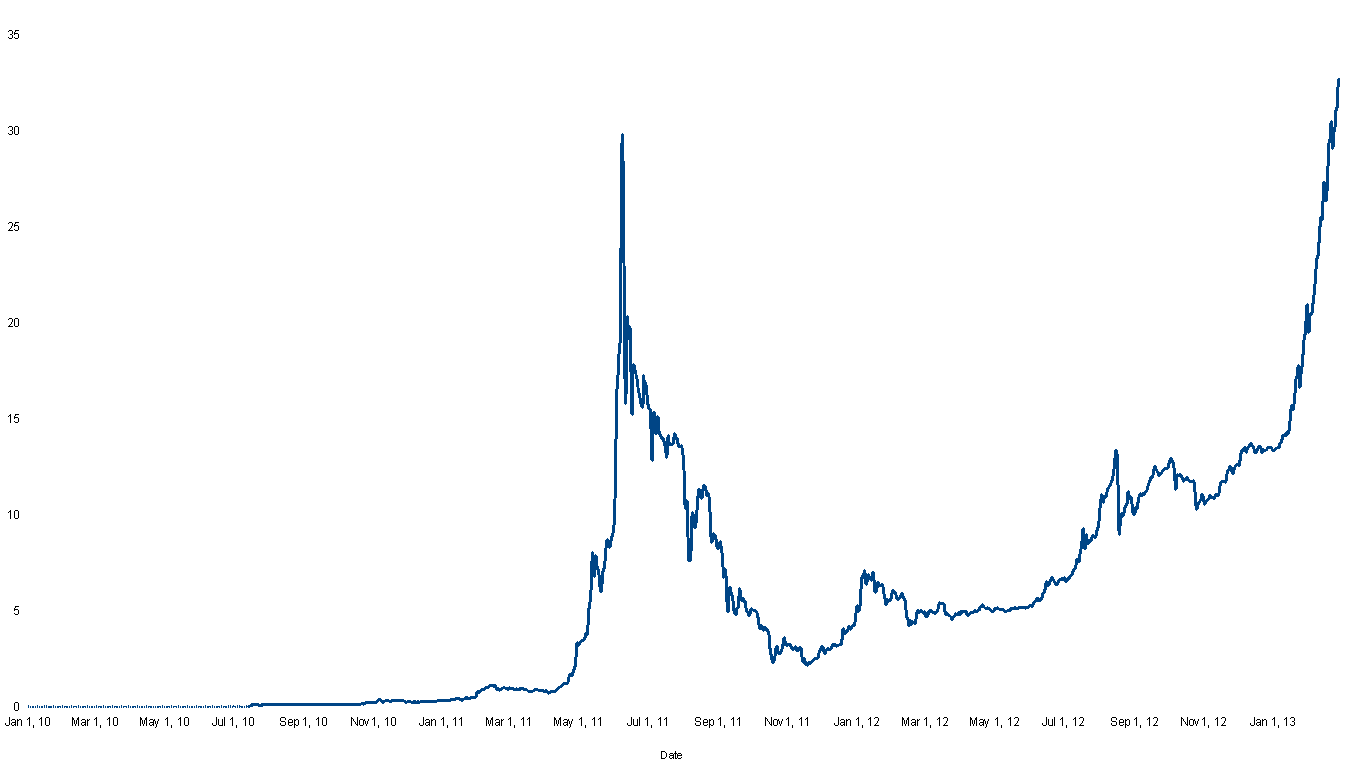
\includegraphics[width=0.8\textwidth]{figures/bitcoin_price.png}
        \column{0.5\textwidth}
        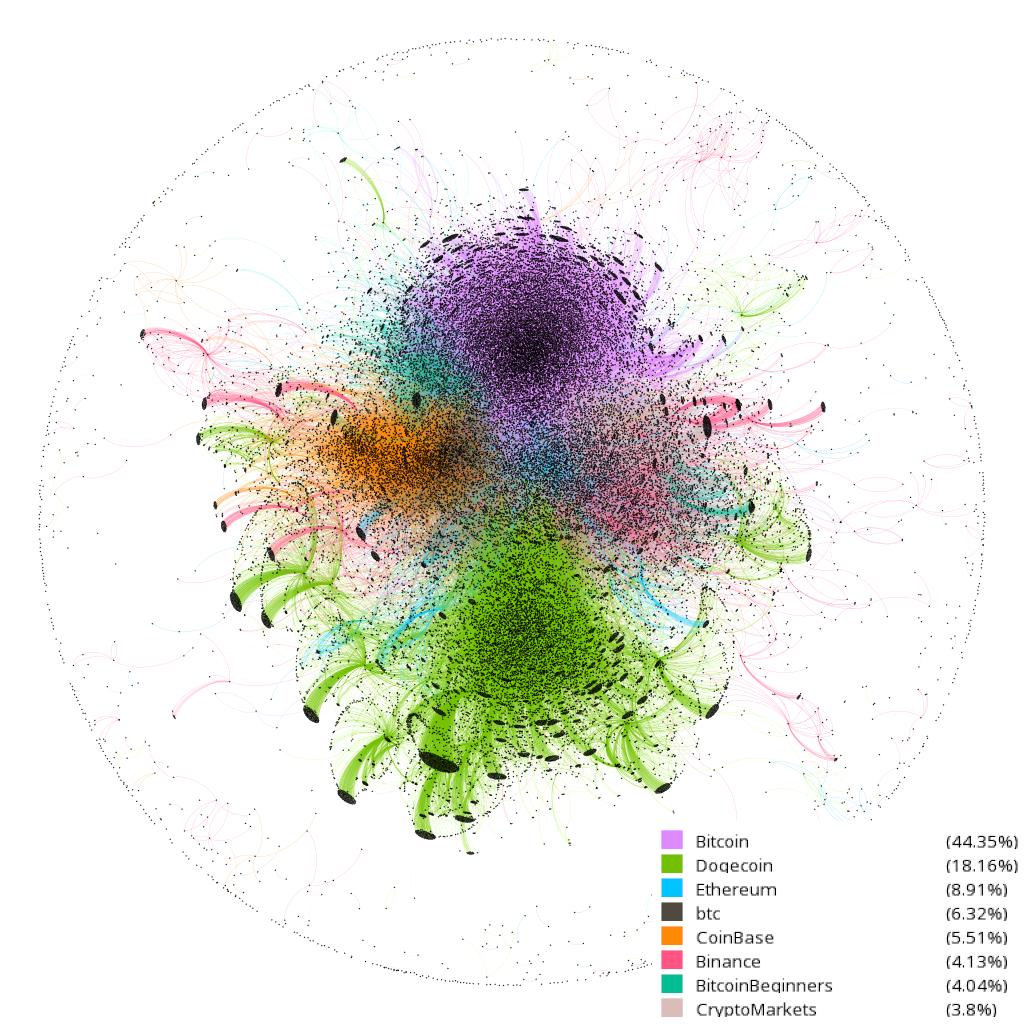
\includegraphics[width=0.8\textwidth]{figures/subreddits_labelled.png}
    \end{columns}
\end{frame}
\section{Trials and Errors}
\begin{frame}[t]
    \frametitle{Trials and Errors}
            The original idea was to perform Sentimental Analysis (SA) on Tweets.
                \vspace{2.0cm}
    \begin{columns}
        \column{0.5\textwidth}
        \begin{itemize}
            \item The Twitter API is unfortunately very limited.
            \item[$\implies$] We took Reddit as a Social Network instead.
        \end{itemize}
        \column{0.5\textwidth}
        \begin{itemize}
            \item Reddit is less suitable to perform Sentimental analysis.
            \item[$\implies$] We decided to analyse the network and find interesting results as well as correlation between subreddit's activity and Bitcoin price.
        \end{itemize}

    \end{columns}
\end{frame}
\section{Data collection}
\begin{frame}[t]
    \frametitle{Data collection}
    \vspace{1.0cm}
    \begin{columns}
        \column{0.4\textwidth}
        \begin{itemize}
            \item We used Reddit API for data collection.
            \item API calls are performed by a bot running every 20 minutes on several Cryptocurrency related subreddits.
            \item Storage is optimal in a JSON format because of Reddit comment structure.
        \end{itemize}
        \column{0.6\textwidth}
        \hspace{1.0cm}
        
\includegraphics[width=0.5\textwidth]{figures/reddit_logo.png}
    \end{columns}
\end{frame}
\section{Data Models}
\begin{frame}[t]
    \frametitle{Data Models}
\end{frame}
\section{Analysis}
\begin{frame}[t]
    \frametitle{Analysis}
    \framesubtitle{Power law distribution}
\end{frame}
\begin{frame}[t]
    \frametitle{Analysis}
    \framesubtitle{PageRank}
\end{frame}
\begin{frame}[t]
    \frametitle{Analysis}
    \framesubtitle{Correlation to price development}
\end{frame}
\section{Homemade implementation}
\begin{frame}[t]
    \frametitle{Homemade implementations}
    \framesubtitle{PageRank}
    
\end{frame}
\begin{frame}[t]
    \frametitle{Homemade implementations}
    \framesubtitle{Louvain}
    
\end{frame}
\section{Discussion}

\end{document}
